\documentclass[12pt]{article}
\author{Adam A. S. Green}
\title{Summer NSERC Research Project 2010-2011}
\usepackage{amssymb, amsmath, float, subfig,caption, hyperref}
\usepackage{epsfig, graphicx}
\usepackage{fullpage}
\usepackage{verbatim}
\usepackage{setspace}
\usepackage{listings}
\begin{document}
\bibliographystyle{plain}

\maketitle
\doublespacing
\section{Introduction}

This report aims to show that under certain circumstances, a neutral bose system can look like
a charged, fermi system.

I will be showing circumstantial evidence, as well as definative results that show numerically
show that similar behaviour is seen.

\subsection{Problems}
I will list the problems/confusions/ambiguities here.

\subsubsection{Prefactor}
The prefactor isn't correct.
The kubo calculation that I am using looks like:
\begin{equation}
\label{kubo_alpha}
(\sigma^{xy})_\alpha = - i L^2 \hbar \sum_{\beta \neq \alpha} \frac{<\alpha|j_x|\beta > <\beta|j_y|\alpha> - <\alpha|j_y|\beta><\beta|j_x|\alpha>}{[E_\beta(t)-E_\alpha(t)]^2}
\end{equation}
with the $\vec{j}$ equal to:
\begin{align*}
j_x & = \sum_{h=0}^{Q-1}-2 \sin(k^0_x + 2 \pi \frac{P}{Q}h)a(k_x^0,k_y)a^\dagger(k_x^0,k_y)\\
j_y &= \sum_{h=0}^{Q-1} -i\exp(k_y)a(k_x-2 \pi \frac{P}{Q}(h-1),k_y)a^\dagger(k_x^0,k_y)+i\exp(ik_y)a(k_x+2 \pi \frac{P}{Q}(h+1),k_y)a^\dagger(k_x,k_y)
\end{align*}
The actual code I used is here:
\lstset{language=Fortran, breaklines=true}
The part that will calculate $j_x$:
\begin{lstlisting}
!FORTRAN J_X CALCULATOR!!!!!!!!!!
do m = 1,Q
	if(xx(i,m) .ne. 0)THEN
	!interactions have been added
	Hx(i,k) = Hx(i,k) -1.0*dble(xx(i,m))*2.0*sin(kx+2.0*PI*dble(P)*dble(m)/dble(Q))
	ENDIF
ENDDO
\end{lstlisting}

Where xx(i,m) contains the prefactor due to the
bose enhancement factor, P/Q is the magnetic flux, and
Hx(i,k) is the matrix that will hold the representation
of the $j_x$ operator. This matrix will be diagonal.
The matrix is also summed over i,k. So the code snippet
above will calculate the $j_x$ matrix element (i,k). 


The part that calculates $j_y$:
\begin{lstlisting}
!FORTRAN J_Y CALCULATOR!!!!!!!!!!!
!pseudo code: IF (CONDITIONS SUCH THAT i,k = i,i+1) THEN
Hy(i,k) = Hy(i,k)+J*prefac*exp(J*ky)
 !pseudo code: IF (CONDITIONS such that i,k = i,i-1) THEN
Hy(i,k) = Hy(i,k)-J*prefac*exp(-J*ky)
\end{lstlisting}


So, when those conditions are used, when I actually calculate the Kubo formula, Eq. \eqref{kubo_alpha} for a single alpha
and then sum over all alphas, I get:
\begin{equation}
\label{result}
\sum_{\alpha} \frac{\sigma^{xy}_\alpha }{L^2 \hbar} = M \frac{L^2Q}{ 2 \pi}
\end{equation}
where $M \in \mathbb{Z}$, it is the quantized kubo conductance that I am looking for. However, the code gives me this funny prefactor. So
when I divide my results by $L^2 Q$ and multiply by $2 \pi$, I get the predicted integer value. Note: on the left hand side, I have
$\frac{\sigma^{xy}_\alpha }{L^2 \hbar} $ because my code actually only evaluates: $$ \sum_{\beta \neq \alpha} \frac{<\alpha|j_x|\beta > <\beta|j_y|\alpha> - <\alpha|j_y|\beta><\beta|j_x|\alpha>}{[E_\beta(t)-E_\alpha(t)]^2}$$

\subsection{To Do}

\section{Main Evidence}
This section will be showing the evidence of a gap in the energy. Show the graphs that
show the single particles occupation as a function of the temperature. Show that the system
really behaves like a fermi system, and that a gap will always been seen to exist at low
temperatures.
\subsection{Energy Gaps}
Figure 1: Intro figure showing the energy levels for the single particle.
Link to appendix that shows how to use the code to generate this figure.
Also include the derivation of the hamiltonian in the appendix.


\begin{figure}[H]%{R}{0.5\textwidth}
 	\centering
        \scalebox{.9}{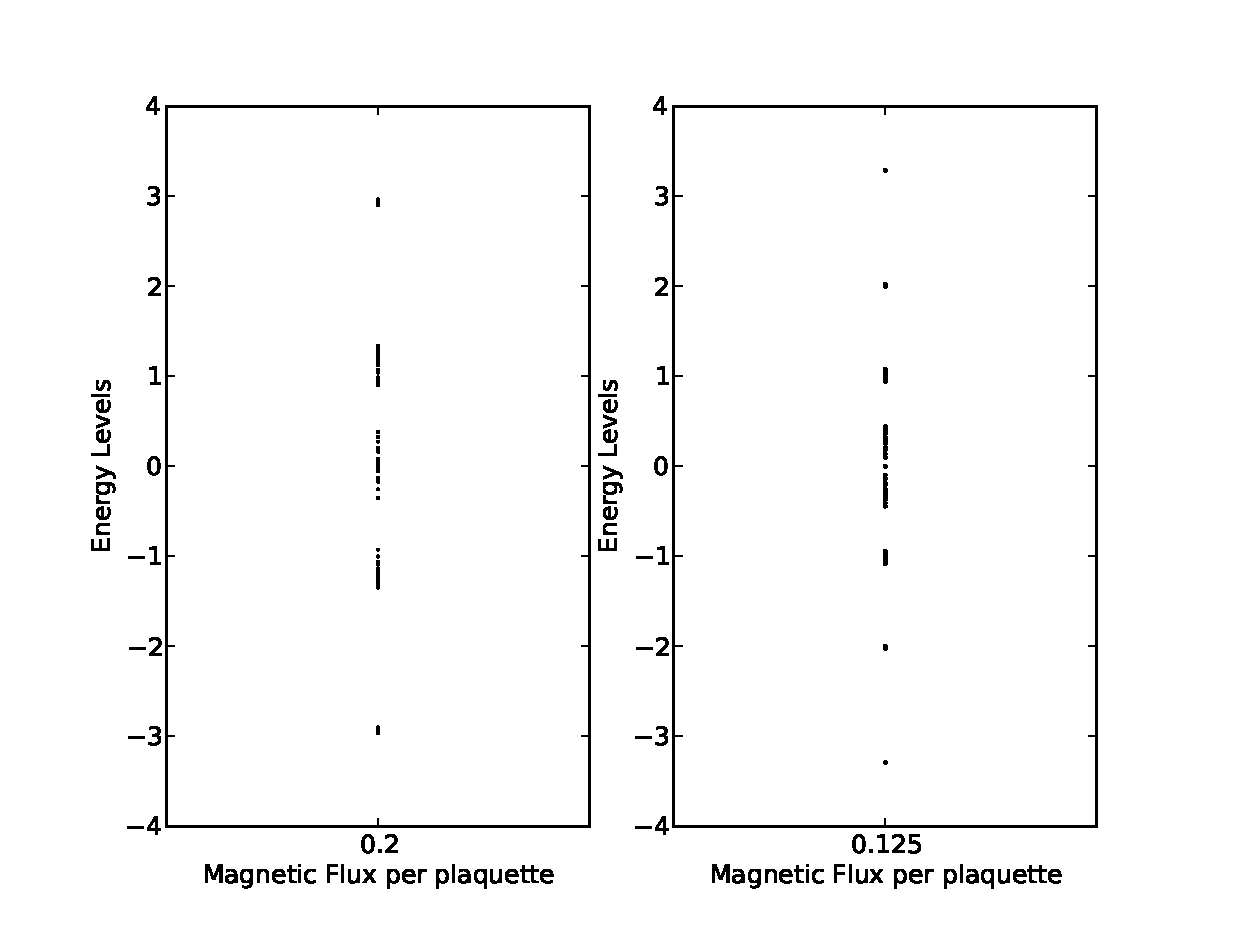
\includegraphics{./figs/fig1/spectrumF5F8}}
          \caption{This shows the spectrum of a 2-D system of electrons in a periodic
		  potential with a magentic field perpendicular to the plane of the system. I have isol
		  the interesting cases where the Flux per plaquette is 1/5 and 1/8. These
		  values both have nice structure, as they clearly have a gap between two of
		  the lowest energy subbands.} 
          \label{intial spectrum}
\end{figure}


Figure2:
Show the occupation of the first and second band as a function of temperature.
Show that for N=1, N=2, N=3, the system behaves exactly the same. And show that
there exists a range of temperatures that illustrate that there is a small gap present at
those low temperature.

\begin{figure}[H]%{R}{0.5\textwidth}
 	\centering
        \scalebox{.9}{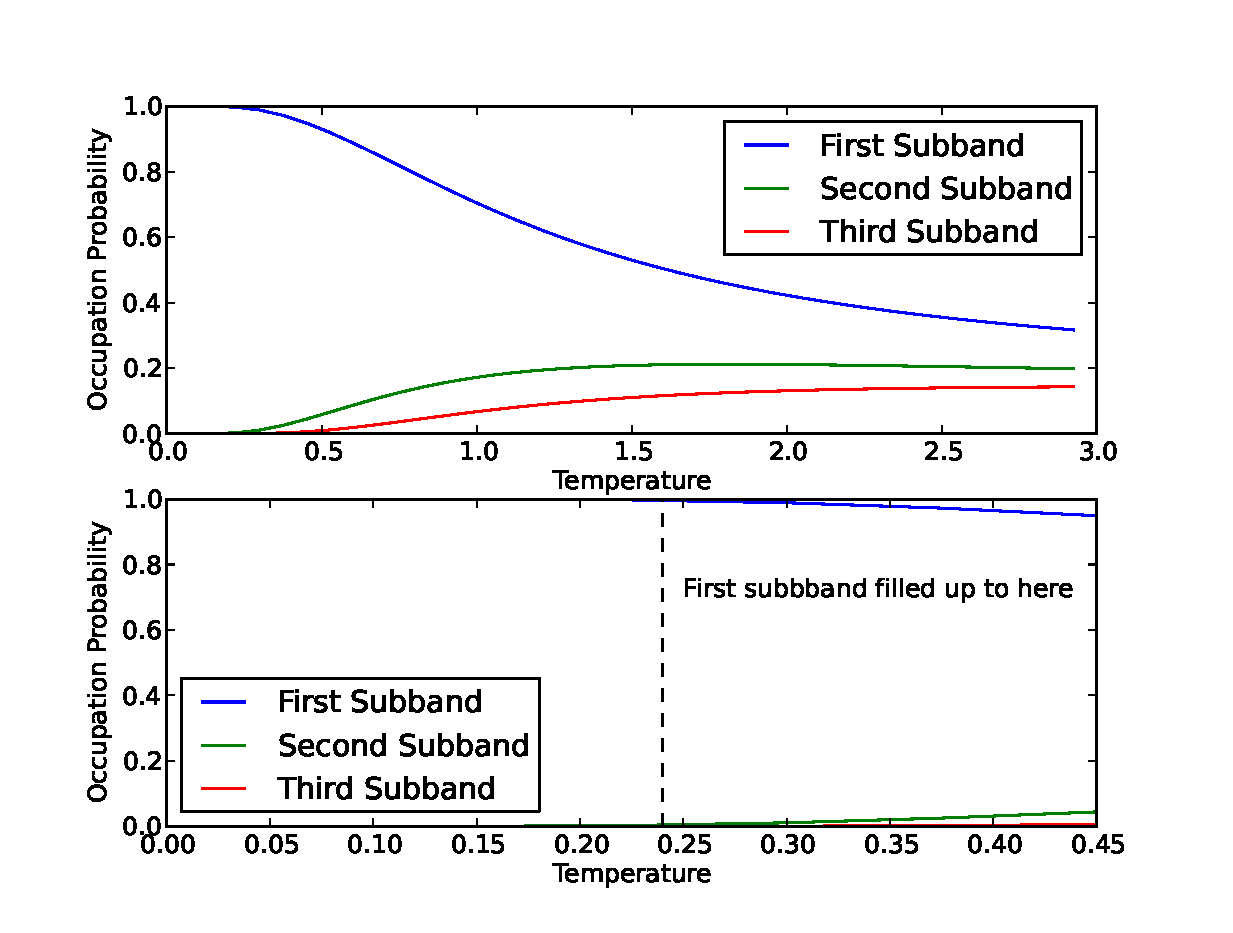
\includegraphics{./figs/fig2/occupProb}}
          \caption{The occupation as a function of temperature. Note how the
		  first band dominates the occupation factor until the dashed line. 
	  This is thought to be because the gap is large enough that the bosons
		  cannot become thermally excited enough to occupy the second subband,
		  but they have more then enough energy to equally thermally occupy the
		  first band.} 
         \label{Occup}
\end{figure}


\subsection{Problems}
\textbf{P:}I am explicitly using a fixed number $N$ of particles, but the bose distribution (which I use for the statistics) requires
a grand canonical ensemble. 
\text{A:} Valid problem. Need to see how the occupation of the levels works in the grand canonical system. See if there are platueas in the
average energy of the system when the temperature is increased. The specific heat of the system will also give indicition of energy gaps.


So, I have know shown evidence that a gap is present at low temperatures. Also, talk about how
if interactions are off that a gap must always be present at low temperatures, just because of the way the single particles combine. However, the subbands will get bigger.

\section{Hall Conductance for Fermions}
I need to at least replicate the results for the fermion system with
the code that I had generate. These results are shown below, as well
as the scaling with different parameters in my system.
These results correspond to the following formula:
\begin{equation}
\label{fermiForm}
\sigma_F = \frac{2 \pi}{L^2 Q} f(\alpha)\sum_{\alpha}\sum_{\beta \neq \alpha} \frac{<\alpha|j_x|\beta > <\beta|j_y|\alpha> - <\alpha|j_y|\beta><\beta|j_x|\alpha>}{[E_\beta(t)-E_\alpha(t)]^2}
\end{equation}
with the $\vec{j}$ equal to:
\begin{align*}
j_x & = \sum_{h=0}^{Q-1}-2 \sin(k^0_x + 2 \pi \frac{P}{Q}h)a(k_x^0,k_y)a^\dagger(k_x^0,k_y)\\
j_y &= \sum_{h=0}^{Q-1} -i\exp(k_y)a(k_x-2 \pi \frac{P}{Q}(h-1),k_y)a^\dagger(k_x^0,k_y)+i\exp(ik_y)a(k_x+2 \pi \frac{P}{Q}(h+1),k_y)a^\dagger(k_x,k_y)
\end{align*}
and where $f(\alpha$ is the fermi occupation. Note, I wrote
$\sigma_F$ istead of the Hall current because I have
several unaccounted for prefactors. This is the raw equation I used
to generate the graphs. 
\begin{figure}[H]%{R}{0.5\textwidth}
 	\centering
        \scalebox{.9}{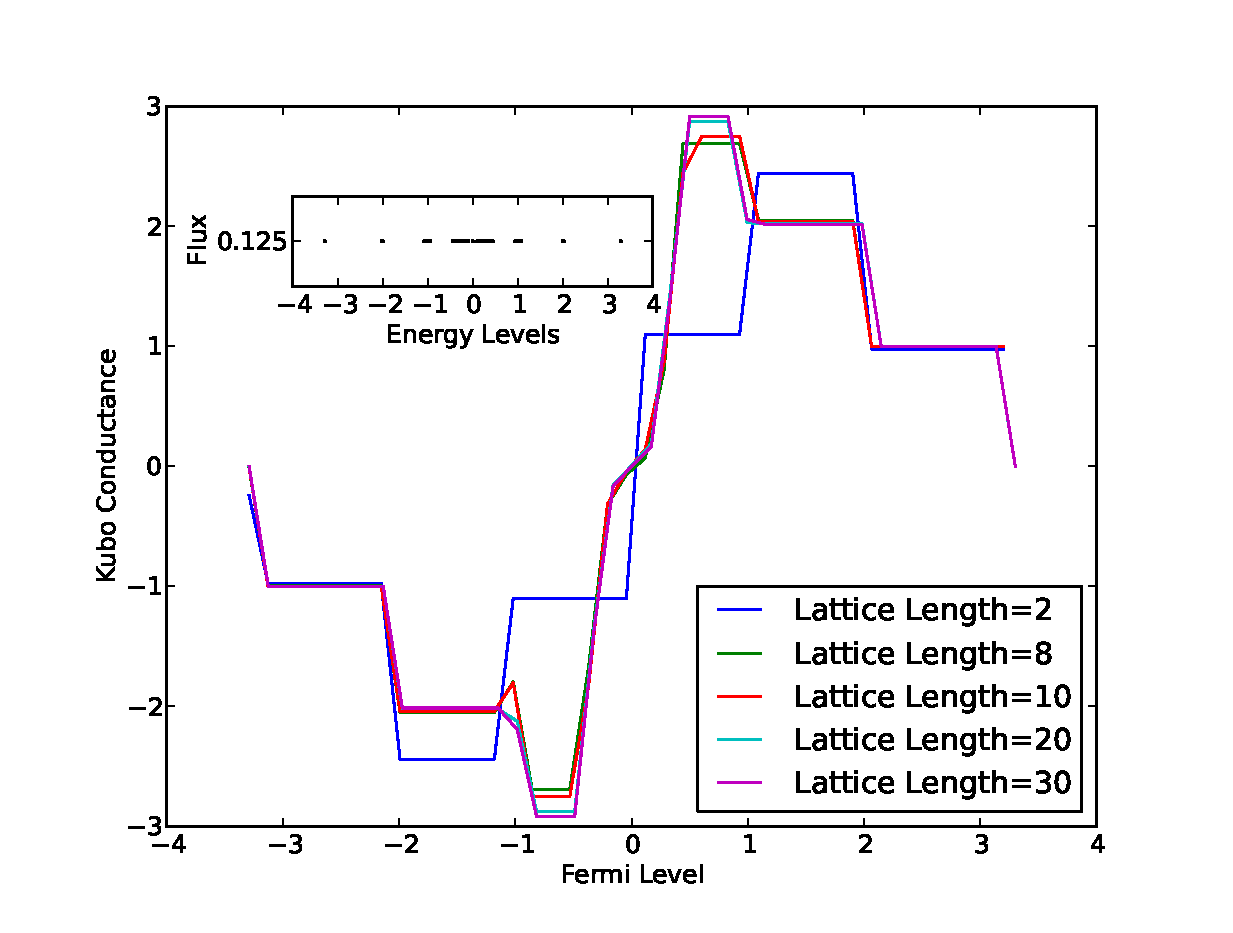
\includegraphics{./figs/fig3/kScalingKubo}}
		\caption{As the size of the lattice is increased, it seems that the system is converging to the quantum hall effect. The predicted values should be platuaus seen at (-1,-2,-3,3,2,1). The scaling behaviour
		seen can be explained by noting that the kubo formula is a
		cumulative sum over the contributions. Each subband should
		contribute -1 (at least for the first three platueas). Therefore, if the calculation of the kubo for each subband is independant, the third platuea should have 3*(K). If we treat K as a measured value, the error will be: $\Delta K_3 \approx 3 K_1$. So we can predict that
		the program will need more precision in the subbands to
		obtain a value that converges to -3, simply because the
		error propogation involved in adding the contributions from
		the subbands together}
         \label{QScalingQHE}
\end{figure}
\begin{figure}[H]%{R}{0.5\textwidth}
 	\centering
        \scalebox{.9}{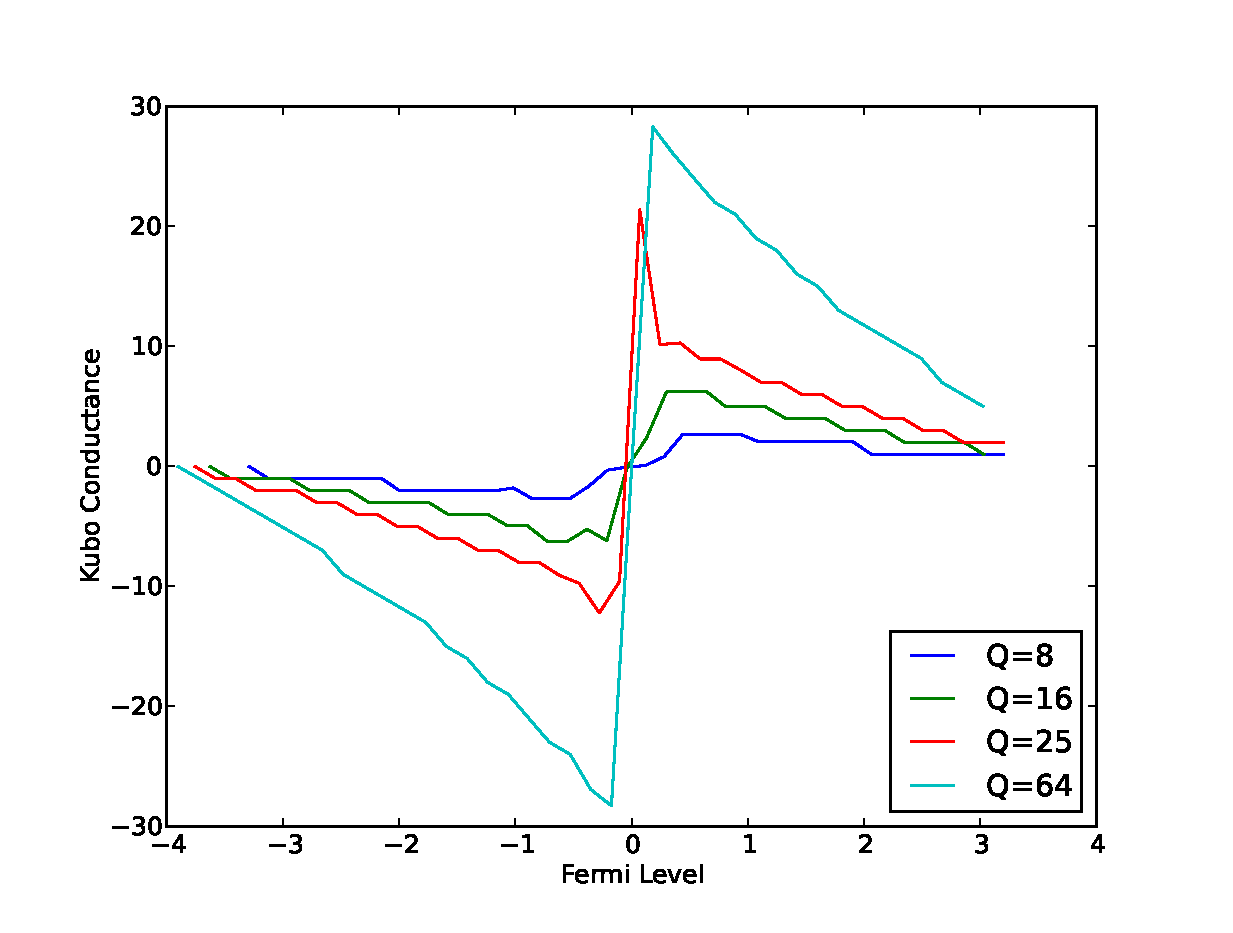
\includegraphics{./figs/fig4/QScalingKubo}}
		\caption{This figure isn't as important as Figure~\ref{kScalingQHE}, but it is interesting to see what happens for different Q's. I tried out several different ones, and one can see quantization (platueas) for several other values. This seems promising, as being able to
		see quantization at lower magnetic fields is always good. Future work would be to apply the bose case to these lower magnetic fields and explore them more.}
         \label{QScalingQHE}
\end{figure}
\section{Bose QHE}
After confirming that my code worked by replicating the QHE shown in 
Figures~\ref{QScalingQHE} and \ref{kScalingQHE}, I moved onto trying to
replicate the conditions of the Fermi case, using bosons.

The idea is to have Boson's at finite temperature. Boson's at high temperature essentially act like Boltzmanon's: they will smear out over the
energy levels equally. However, if the energy levels being smeared over are actually a subband, and if there is a high enough energy level gap
to the next subband, then the bosons will smear out equally over the lwest subband, while note occupying the second one. This essentially mimics a Fermion system where each energy level in the lowest subband is filled, but no other energy level is occupied; ie. the fermi energy is a little above the first subband. Note, that to get a direct analogy,
the bose density ($\frac{\text{N of boson's}}{N of states}$) has to be approximately equal to 1.

However, we see exactly the conditions described above in Figure~\ref{Occup}. With this system, I used the kubo formula to calculate the
hall conductance.
\begin{equation}
\label{bosonForm}
\sigma_B = \frac{2 \pi}{L^2 Q} \frac{b(\alpha)}{N}\sum_{\alpha}\sum_{\beta \neq \alpha} \frac{<\alpha|j_x|\beta > <\beta|j_y|\alpha> - <\alpha|j_y|\beta><\beta|j_x|\alpha>}{[E_\beta(t)-E_\alpha(t)]^2}
\end{equation}
with the $\vec{j}$ equal to:
\begin{align*}
j_x & = \sum_{h=0}^{Q-1}-2 \sin(k^0_x + 2 \pi \frac{P}{Q}h)a(k_x^0,k_y)a^\dagger(k_x^0,k_y)\\
j_y &= \sum_{h=0}^{Q-1} -i\exp(k_y)a(k_x-2 \pi \frac{P}{Q}(h-1),k_y)a^\dagger(k_x^0,k_y)+i\exp(ik_y)a(k_x+2 \pi \frac{P}{Q}(h+1),k_y)a^\dagger(k_x,k_y)
\end{align*}
and where $b(\alpha$ is the bose occupation, and $N$ is the number of particles.  Note, I wrote
$\sigma_B$ istead of the Hall current because I have
several unaccounted for prefactors. This is the raw equation I used
to generate the graphs. 
\begin{figure}[H]%{R}{0.5\textwidth}
 	\centering
        \scalebox{.9}{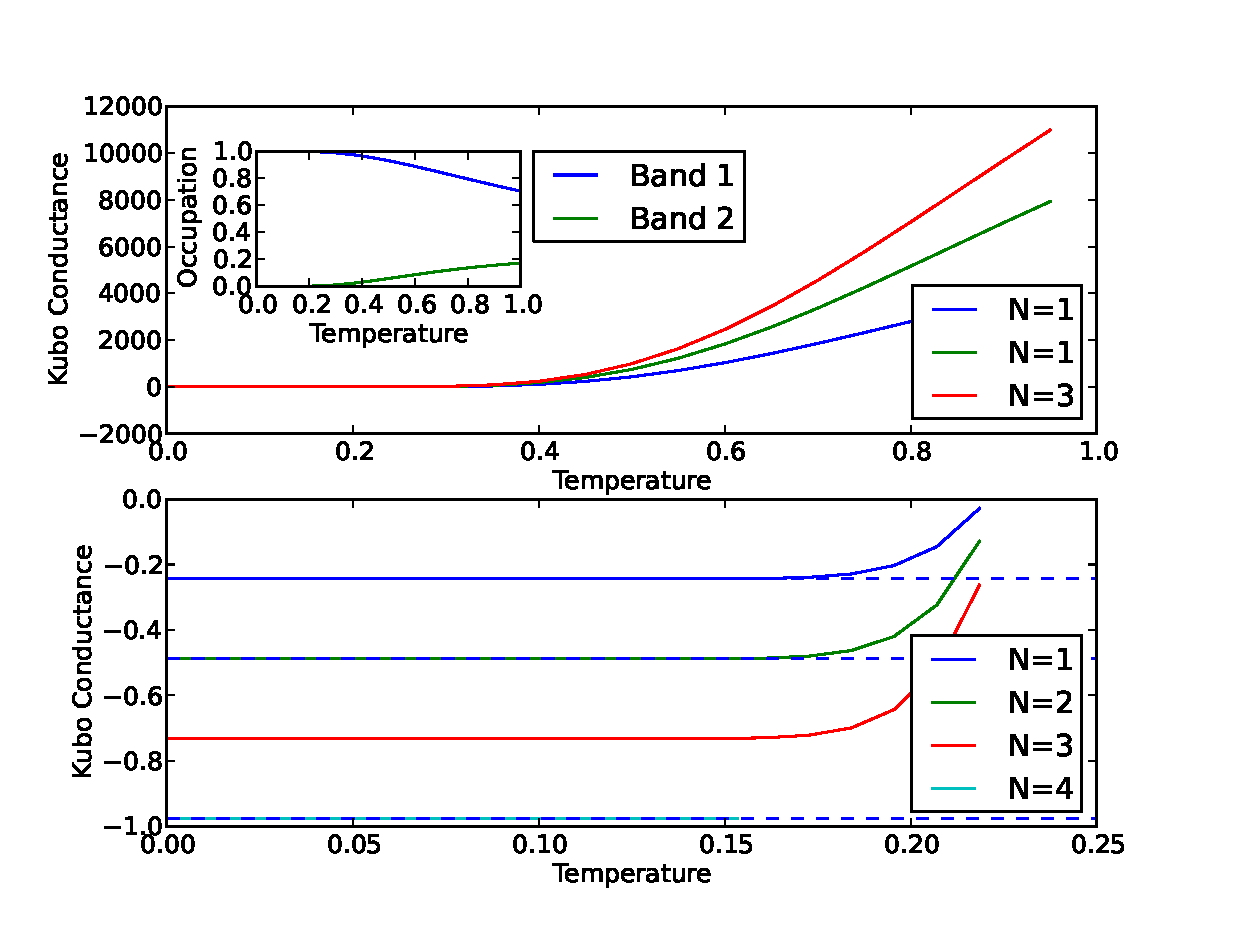
\includegraphics{./figs/fig5/QuantizedBoseGraphsBigAndSmallTInset}}
		\caption{The first graph shows what happens at a large temperature range. The second graph zooms into low temperature, and, as you can see the hall effect is quantized. The dashed lines represent the hall conductance calculated for an equivalent $N$ number of fermions. So the
		$N=1$ boson and fermi line up, and so on. Because of a degeneracy in the energy levels, my code jumped from 2 fermions to 4, which is why there is no $N=3$ fermion to compare to the boson. The inset
		shows the occupation of the first two subbands.}
		\label{main}
\end{figure}
\section{Derivations}
\subsection{Kubo Derivation (1)}
The first way I derived the kubo formula was by using the argument from
Mahan. First calculate the polarization operator, and then the particle
current operator is the commutator of the polarization operator with
Hamiltonian, multiplied by i.
\[
\label{j_def}
\hat{j} = i[H,P]
\]
P is given as:
\begin{align}
\hat{P} &= \vec{r} \hat{n}(x,y) \\
\hat{P} &= \vec{r} \hat{a(x,y)} \hat{a(x,y)}^\dagger
\end{align}
and the Hamiltonian is:
\begin{align}
\hat{H} &=  -\tau \sum_{i} \sum_{j=0}^3 \hat{a}_i \hat{a}_{i+\delta_j} e^{i \Theta_j}\\
		&= -\tau \sum_{x} \sum_{y} \sum_{j=0}^3\hat{a}_{x,y} \hat{a}_{x+T_j, y+P_j} e^{i S(x) P_j}
		&\exists T = (-d,d,0,0), \exists P = (0,0,-d,d), \exists S(x) = 2 \pi\frac{P}{Q}x
\end{align}
The above notation is a bit confusing, but the rational is as follows.
The $j$ index indicts a hopping term. So the $T$ vector is a hopping xvector, $d$ is
the lattice spacing. It can hop in the -1x, 1x directionsx. Now, the $P$ vector is the same, but the hopping is
in the y direction. (Sorry for the confusion, but $\hat{P} \neq P$, I wanted to be consistant with my labbook. However, the particle will gain phase only if hops in the y directions. So the $P$ vector is also the phase vector. You gain phase only when you are hopping in the plus-y/minus-y directions. 

$\Theta$ was also expanded out in terms of the prefactor $S(x)$ and the phase vector $P$, ie. $\Theta_j = S(x)P_j$.

Using these expressions for the Hamiltonian and the Polarization operator, Eq. \eqref{j_def} takes the form:
\begin{align}
\hat{j} & = i\left[\hat{H}, \hat{P}]\right]\\
		& = -\tau \sum_{x,y,x',y'} \sum_{j=0}^3\left[\hat{a}^\dagger_{x,y} \hat{a}_{x+T_j, y+P_j} e^{i S(x) P_j},  \vec{r'} \hat{a}^\dagger_{x',y'} \hat{a}_{x',y'}\right] 
\end{align}
Now using the following commutator identities:
\begin{align}
[\hat{A}, \hat{B}\hat{C}] = [\hat{A},\hat{B}]\hat{C} + \hat{B}[\hat{A},\hat{C}], \qquad [\hat{A} \hat{B},\hat{C}] = [\hat{A},\hat{C}]\hat{B} + \hat{A}[\hat{C},\hat{B}]\\
\end{align}
we can expand out the current operator equation to obtain:
\begin{align}
	\hat{j}	& =  -\tau \sum_{x,y,x',y'} \sum_{j=0}^3\sum_{x'}  [\hat{a}^\dagger_{x,y},\vec{r}\hat{a}^\dagger_{x',y'}\hat{a}_{x',y'}]\hat{a}_{x+T_j, y+T_j} e^{ i S(x) P_j}+\hat{a}^\dagger_{x,y}[\hat{a}_{x+T_j, y+T_j} e^{i S(x) P_j},\vec{r}\hat{a}^\dagger_{x',y'}\hat{a}_{x',y'} ] \\     
	& =  -\tau \sum_{x,y,x',y'} \sum_{j=0}^3[ \hat{a}^\dagger_{x,y} ,\vec{r'}\hat{a}^\dagger_{x',y'}]\hat{a}_{x',y'} \hat{a}_{x+T_j, y+T_j} e^{i S(x) P_j}+ \vec{r'}\hat{a}^\dagger_{x',y'}[ \hat{a}_{x,y} , \hat{a}_{x',y'}] \hat{a}_{x+T_j, y+P_j} e^{i S(x) P_j}\\
	&\qquad +\hat{a}^\dagger_{x,y}[ \hat{a}_{x+T_j, y+P_j} e^{ i S(x) P_j},\vec{r'}\hat{a}^\dagger_{x',y'}]\hat{a}_{x',y'} +\hat{a}_{x,y}\vec{r'} \hat{a}^\dagger_{x',y'}[ \hat{a}_{x+T_j, y+P_j} e^{i S(x) P_j},  \hat{a}_{x',y'}] \\
	& = 0 + \vec{r'}\hat{a}_{x',y'}(-\delta_{x,x'}\delta_{y,y'}) \hat{a}_{x+T_j, y+P_j} e^{i i S(x) P_j}+\hat{a}_{x,y}(\delta_{x+T_j,x'} \delta_{y+P_j,y'}) \hat{a}_{x',y'} e^{i S(x) P_j} \vec{r} +0
\end{align}
Summing over $x'$ and $y'$ gets rid of the deltas and leaves us with:
\begin{align}
 \hat{j} & =-\tau \sum_{x,y} \sum_{j=0}^3 \left( -
 \begin{pmatrix}
 	x \\
	y \\
	\end{pmatrix}
\hat{a}_{x,y}^\dagger \hat{a}_{x+T_j, y+P_j} e^{i S(x) P_j}+
 \begin{pmatrix}
 	x+T_j \\
	y +P_j\\
	\end{pmatrix}
\hat{a}_{x,y}^\dagger \hat{a}_{x+T_j, y+P_j} e^{i S(x) P_j}\right)\\
		&= -\tau \sum_{x,y} \sum_{j=0}^3 
		\begin{pmatrix}
			T_j \\
			P_j\\
		\end{pmatrix}\hat{a}_{x,y}^\dagger\hat{a}_{x+T_j, y+T_j} e^{i i S(x) P_j} 
\end{align}
\textbf{NOTE: I think I have made a mistake with the sign. I think
the it is supposed to be a $+\tau$ when you originally solve for the
j operator as the commutator. I think that is what happens in Mahan, it switches sign from the way the Hamiltonian is. }
Now, we use the fourier series to transform to $k$-space.

Anyway, the j current operator, using this setup, becomes:
\begin{align}
	\hat{j}	&= -i\tau \sum_{x,y} \sum_{j=0}^3 
		\begin{pmatrix}
			T_j \\
			P_j\\
		\end{pmatrix}\hat{a}i^\dagger_{x,y}\hat{a}_{x+T_j, y+T_j} e^{i  S(x) P_j} \\
		\end{align}



Current Problems: The prefactor doesn't seem to work. I seem to be
grossly overcounting it. If I am just using the Fourier transform, 
as I was originally going to do, then I will only have the $\sqrt{2 \pi}$ which isn't what I want either.


Then we can use the discrete fourier transform. This is the key point!

The following are definitions of the terms that I will be using:
\begin{align*}
d &:= \text{spacing of crystal sites in position-space}\\
2N &:= \text{The number of crystal sites in position-space}\\
L &:= \text{The length of the lattice in position-space}\\
&\qquad \qquad \therefore L = (2N) a\\
h &:= \text{rows of crystal lattice sites in k-space}\\
d &:= \text{columns of crystal lattice sites in k-space}
\end{align*}
With these definitions, and using the discrete Fourier transform, I can
write the anihilation operator at lattice point $(n,m)$ in position-space:

\begin{align*}
c_{nm} &= \frac{1}{(2N)^2} \sum^{2N-1}_{h=0} \sum^{2N-1}_{b=0} \exp\left[-\frac{2 \pi i}{2N}(bm+hn)\right] c_{h,b}\\
c^\dagger_{n+T_j/d, m+P_j/d} & = \frac{1}{(2N)^2} \sum^{2N-1}_{h=0} \sum^{2N-1}_{b=0} \exp\left[-\frac{2 \pi i}{2N}(b(m+P_j/d)+h(n+T_j/d))\right] c^\dagger_{h,b}
\end{align*}

The current operator becomes:
\begin{multline}
\hat{j} =\-i\tau sum^{2N-1}_{n,m=0} \sum_{j=0}^3
		   \begin{pmatrix}
			T_j \\
			P_j\\
		\end{pmatrix}
\frac{1}{(2N)^4} \sum^{2N-1}_{h,h'=0} \sum^{2N-1}_{b,b'=0}  a^\dagger_{h,b} e^{-\frac{2 \pi i}{2N}bm}  e^{-\frac{2 \pi i}{2N}hn} a_{h',b'} e^{\frac{2 \pi i}{2N}b'(m+P_j/d)}  e^{\frac{2 \pi i}{2N}h'(n+T_j/d)} e^{i S(n) P_j} 
\end{multline}

\begin{multline}
\hat{j} =  -i\tau \sum^{2N-1}_{m,n} \sum_{j=0}^3 \begin{pmatrix}
			T_j \\
			P_j\\
		\end{pmatrix}  
\frac{1}{(2N)^4} \sum^{2N-1}_{h,h'=0} \sum^{2N-1}_{b,b'=0}  a_{h,b} e^{ \frac{2 \pi i}{2N} b'P_j/d}e^{\frac{2 \pi i}{2N} h'T_j/d} e^{-\frac{2 \pi i}{2N}(b-b')m}  e^{-\frac{2 \pi i}{2N}(h-h'-S(n)P_j{n})n} a^\dagger_{h',b'}  \\
\end{multline}
We now expand out the sum over j, as there will be multiple times when
the orthogonality condition used by the discrete Fourier transform is met:
\begin{multline}
\hat{j} =  -i\tau \sum^{2N-1}_{m,n} 
\frac{1}{(2N)^4} \sum^{2N-1}_{h,h'=0} \sum^{2N-1}_{b,b'=0} \left( \begin{pmatrix}
			-d \\
			0\\
		\end{pmatrix}  e^{-h'\frac{2 \pi i}{2N}}  e^{-\frac{2 \pi i}{2N}(b-b')m}  e^{-\frac{2 \pi i}{2N}(h-h')n}a^\dagger_{h,b} a_{h',b'}\right.\\
		+  \begin{pmatrix}
			d \\
		0\\
		\end{pmatrix}  e^{h'\frac{2 \pi i}{2N}}  e^{-\frac{2 \pi i}{2N}(b-b')m}  e^{-\frac{2 \pi i}{2N}(h-h')n} a^\dagger_{h,b}a_{h',b'}
		+  \begin{pmatrix}
			0 \\
		-d\\
		\end{pmatrix}  e^{-b'\frac{2 \pi i}{2N} }  e^{-\frac{2 \pi i}{2N}(b-b')m}  e^{-\frac{2 \pi i}{2N}(h-h'+2 \pi P/Q)n} a^\dagger_{h,b}a_{h',b'}\\
		\left.+ \begin{pmatrix}
			0 \\
		d\\
		\end{pmatrix}   e^{b'frac{2 \pi i}{2N}'} e^{-\frac{2 \pi i}{2N}(b-b')m}  e^{-\frac{2 \pi i}{2N}(h-h'-2\pi P/Q)n} a^\dagger_{h,b}a_{h',b'} \right) 
\end{multline}
Summing over the m (y direction) will present no problem. Realizing that
$\sum_m^{2N-1} e^{\frac{2 \pi i}{2N}(b-b')m}$ will only be equal to one if $b=b'$ mod $2 \pi$, shown below:

Let r be defined as follows:
\begin{gather*}
r = \exp[ \frac{2 \pi i}{2N}(b-b')] \\ 
\text{If b=b', then r =1 and the sum over r will give:$ \sum_{m=0}^{2N-1} r^m =2N$} \\ 
\text{If b $\neq$ b' then, using induction:}\\
p = \sum_{m=0}^{2N-1} r^m = 1+r+r^2+...r^{2N-1}\\
rp = r+r^2+...+r^{2N} = p+r^{2N} -1\\
\therefore rp -p = r^{2N} -1, \qquad \text{factoring and dividing gives:}\\
p  = \frac{r^{2N} -1}{r-1}
\text{But, $r^{2N} = \exp[2 \pi i(b-b')m] =1, \; \; \therefore p =0$}
\end{gather*}
So this gives the 
unscaled orthogonality condition.

We can now use this orthogonality condition and sum over n and m to reduce our sum: first
summing over m gives:
\begin{multline}
\hat{j} = -i\tau  
\frac{1}{(2N)^2} \sum^{2N-1}_{h,h'=0} \sum^{2N-1}_{b,b'=0} \left( \begin{pmatrix}
			-d \\
		0\\
		\end{pmatrix} e^{-h'\frac{2 \pi i}{2N}'} e^\dagger_{h,b} \delta_{b,b'} \delta_{h,h'} a_{h',b'}+\begin{pmatrix}
			d \\
		0\\
		\end{pmatrix} 
e^{h'\frac{2 \pi i}{2N}'} a^\dagger_{h,b} \delta_{b,b'} \delta{h,h'} a_{h',b'}  \right. \\
\left.+\begin{pmatrix}
			0 \\
		-d\\
		\end{pmatrix} e^{-b'\frac{2 \pi i}{2N}'} a^\dagger_{h,b} \delta_{b,b'}  \delta_{h,h'+2 \pi P/Q} a_{h',b'}+ \begin{pmatrix}
			0 \\
		d\\
		\end{pmatrix} e^{b'\frac{2 \pi i}{2N}'} a^\dagger_{h,b} \delta_{b-b'} \delta_{h,h'-2\pi P/Q)n} a_{h',b'} \right) 
\end{multline}
Therefore, we can transform the current operator to be in terms of k's
\begin{multline}
\hat{j} =  -\tau 
\frac{1}{(2N)^2} \sum^{2N-1}_{h=0} \sum^{2N-1}_{b=0} \left( \begin{pmatrix}
			d \\
		0\\
		\end{pmatrix} -2 \sin(-h'\frac{2 \pi i}{2N}) a^\dagger_{h,b}  a_{h,b}+\begin{pmatrix}
			0 \\
		-d\\
		\end{pmatrix} ie^{-b'\frac{2 \pi i}{2N}} a^\dagger_{h-2 \pi P/Q,b}  a_{h,b}\right.\\
		\left.+ \begin{pmatrix}
			0 \\
		d\\
		\end{pmatrix} ie^{b'\frac{2 \pi i}{2N}} a^\dagger_{h+2\pi P/Q,b}  a_{h,b} \right) 
\end{multline}
Note, I summed over h in the above, so I was left over with h'. You can rename the dummy variable to h', but I wanted to be pedantic.
We can further transform this into a sum over k, by realizing that we
can define k in terms of the integers:
\[
k_h = \frac{2 \pi h}{QL}, \qquad k_b = \frac{2 \pi b}{L}
\]
Therefore:
\[
h = \frac{k_h QL}{2 \pi}, \qquad b = \frac{k_b L}{2 \pi}
\]
Also,
\[
2N*d = L
\]

\begin{multline}
\hat{j} = -\tau 
\frac{1}{L^2} \sum_{k_h =0}^{\frac{2 \pi (2N-1)}{QL}} \sum_{k_b =0}^{\frac{2 \pi (2N-1)}{L}} \left( \begin{pmatrix}
			d \\
		0\\
		\end{pmatrix} -2 sin(k_x) a^\dagger_{h,b}  a_{h,b}\begin{pmatrix}
			0 \\
		-d\\
		\end{pmatrix} ie^{-k_b} a^\dagger_{k_h-2 \pi P/Q,k_b}  a_{k_h,k_b}\right. \\
		\left.+ \begin{pmatrix}
			0 \\
		d\\
		\end{pmatrix} ie^{k_b} a^\dagger_{k_h+2\pi P/Q,k_b}  a_{k_h,k_b} \right) 
\end{multline}
Changing the bounds of summation, this becomes more familiar:
\begin{multline}
\hat{j} = -\tau 
\frac{1}{L^2} \frac{1}{L^2} \sum_{k_h =\frac{- \pi}{Q}}^{\frac{\pi}{Q}} \left( \begin{pmatrix}
			d \\
		0\\
		\end{pmatrix}- 2 sin(k_x) a^\dagger_{h,b}  a_{h,b}\begin{pmatrix}
			0 \\
		-d\\
		\end{pmatrix} ie^{-k_b} a^\dagger_{k_h-2 \pi P/Q,k_b}  a_{k_h,k_b}\right.\\
		\left.+ \begin{pmatrix}
			0 \\
		d\\
		\end{pmatrix} ie^{k_b} a^\dagger_{k_h+2\pi P/Q,k_b}  a_{k_h,k_b} \right) 
\end{multline}
\textbf{NOTE: I think I have made a mistake with the sign. I think
the it is supposed to be a $+\tau$ when you originally solve for the
j operator as the commutator. I think that is what happens in Mahan, it switches sign from the way the Hamiltonian is. }


However, while this is my best shot at the derivation, it still doesn't
give the right prefactors, so it is probably wrong.
\begin{comment}
%THIS TABLE IS NOW OBSOLETE, USE THE KUBO GRAPHS INSTEAD.
Also, present a table of the quantized values
\section{Table of Kubo Values}
\begin{table}[H]
\begin{tabular}{c|c|c|c|c|c|c|c}
\hline
 	&	N=1 & N =2 &N=3& FERMI N=1&FERMI N=2&FERMI N=3 &FERMI N=4 \\
Q =2& 0.  & 0. &0.& 0.&0.\\
Q =3& -.72175 & -2.8868 &-6.49498 &-.72168&-1.4434&-2.165&-2.88675\\
Q = 4& -.062499 & -.2500 &-5.62504&-.062500&-.12500&-.187500&-.2500\\
Q = 5& -.28410 & -1.1364 & -2.5567&-.28409&-.55817&-.852261&-1.1363\\
Q = 6& -.20351 & -       &- &-.20350&-.40700&-.61051&-.814001 \\
Q = 7 & -.2960 & -1.1841&-2.6643&-.29603 &-.59205 &-.88808 & -1.1841\\
Q = 8 & -.31081 &-1.24319&-&-.31080&-.62161&-1.24322&-1.24322\\
Q = 16& -.63665 & -2.54655 &-&-.63662&-1.2732&-1.90984&-2.5464\\
Q = 32& -1.2731 &-&-1.2732 &-&-2.5464 &-3.8197&-5.0929\\
\end{tabular}
\end{table}
\end{comment}


\section{Conclusion}: Show that regardless of prefactor, the bose case resembles the fermi case
at low temperatures. Think about why it is that N=2 is the best one. Talk about how the scaling
has to be right. You need the bose density to be right. This means having a high particle number
and a low system size. You want the number of bosons in an energy level to be about the number
of energy levels present in the subband. This ensures that the band 'looks' all filled up.

You can see a Quantum Hall effect using boson's at finite temperature. 
\end{document}
\\begin{comment}
\begin{multline}
\hat{j} =\sum_{x,y} \sum_{j=0}^3
		   \begin{pmatrix}
			T_j \\
			P_j\\
		\end{pmatrix}
\frac{1}{b_x  b'_x  b'_y  b_y (2 \pi)^4} \int^{b_x}_0 dk_x \int^{b_y}_0 dk_y a(k_x,k_y) e^{-i\frac{k_x}{b_x}x} e^{-i\frac{k_y}{b_y}y} \int^{b'_x}_0 dk'_x \int^{b'_y}_0 dk'_y \\
a^\dagger(k'_x,k'_y) e^{-i\frac{k'_x}{b'_x}x} e^{-i\frac{k'_y}{b'_y}y'} e^{-iS(x) P_j} 
\end{multline}

Recognizing that there are delta functions in this series, we can rewrite this
as follows:
\begin{multline}
a(x,y) =  \sum_{x,y} \sum_{j=0}^3 \begin{pmatrix}
			T_j \\
			P_j\\
		\end{pmatrix}  
\frac{1}{b'_x b'_y b_x  b_y (2 \pi)^4} \int^{b'_x}_0 dk'_x \int^{b'_y}_0 dk'_y\int^{b_x}_0 dk_x \int^{b_y}_0 dk_y a(k_x,k_y) e^{-i(\frac{k_x}{ b_x}-\frac{k'_x}{ b'_x}-\frac{S(x)}{x})x} \\
e^{-i(\frac{k_y}{ b_y}-\frac{k'_y} {b'_y})y} a^\dagger(k'_x,k'_y)  
\end{multline}


I have another problem now. The goal and the aim is to create delta functions,
so that I can get rid of the $k'$s and simplify things. In order to do that however, I need to use one definition of the delta function as:
\begin{equation}
\delta(x-a) = \frac{1}{L} \int^{L}_0 dx e^i(k-k')\frac{x}{L}
\end{equation}
where, as before, $L$ and $k$ have a 'hidden' $2 \pi$ in them.

The problem is two-fold. First, I do not have an integral, I have a sum.
Second, I do not really know where the sum terminates, which is difficult as
that will determine the $L$ factor. I know that, in principle, it is carried
out to infinity, as the lattice is assumed to have complete translational symmetry. However, I also have periodic boundary conditions and a finite lattice.

I have had several epiphanies. I will write them down before I forget.
1. I can have a continous range of values in the Brilloiun zone. Because
we are not working with position, but explicitly working in momentum
space, creating particles with definite momentum, we can create a particle
with any momentum. However, we are restricting ourselves to looking at the
first translational band. Which means that $-\pi < k_x <\pi$ and $-\pi < k_y < \pi$. However, due to the magnetic field, the brilloiun zone in $k_x$ is split
into $Q$ pieces, but we still sum over them all. We just replace our integral
over all $k_x$ with an integral over the first 'magentic' brilloiun zone, and
then have a sum over j to reach all Q brilloin zones. Although, the sum
over j is already there to deal with the hopping gained by the phase. I will still have to think about that.

2. This means that I was wrongheaded in how I originally did things. The sum over position space has to go over all positions, because that is what is needed 
to create a definite value of k. Also, because we can create a particle
with any value of k in the brilloiun zone, there is no benefit to taking
a small sized system. It just means that we are sampling at a very low rate, this
doesn't reflect the finite size of our crystal.

So, with the thought that we are working in the momentum representation
always in the back of our mind, the definition of the creation operator doesn't
seem so far fetched now:
\begin{equation}
c_{nm} = \frac{1}{(2 \pi))^2} \int^\pi_\pi dk_x \int^\pi_\pi dk_y exp[ i(k_x n+k_ym)] \times c(k_x,k_y)
\end{equation}
This is a bit handwavy, but my reasons are this. You can only create/destroy
a particle in a restriced condition (integer multiple of n in x and m in y).
However, if that is true, then why can you create/destroy a particle in
a continumn of places in kx,ky space?

Anyway, normally, I would expect this integral to be over infinity. To create
a definite particle at a definite position (n,m) it seems that you would be
making a delta function, which means that you need contributions from all
the k's. However, the first puzzle is that the integral is only over the first
translational brilloin zone. Is integrating over the first brilloin zone 
equivalent to summing over infinity? Naivelly, yes. As all the 
pertinant information is contained in the primitive cell (brilloin zone).
However, I feel uneasy as I can't think of a way to prove this. Reducing this
to a single dimension, any integer multiple of the reciprocal primitive lattice
vector will give the primitive lattice vector.
If we are integrating over the reduced brilloin zone, that would make a little
more sense. Is there a mapping between the whole k space and the
reduced brilloin zone that allows you to use an integral?

3. I just had another epiphany. I have been thinking about pseudo momentum
and momentum as the same thing, but they aren't. The brilloiun zone only
described the properties of the crystal. It puts limits on the k vectors,
but it doesn't prescribe their values. The only thing that will determine
the k vectors is the solution to the SWE. So, a crystal can support
a continium of k-vectors
$\exp[i(k_x n)]$ where $k_x$ goes over all space. 
But $\exp[i(k_x n)]=\exp[mi(k_x n)]$ mod $2 \pi$. But this won't
fill up the brilloin zone, it just stacks vector on top of each other.

Okay, this is how I think the derivation goes now:
The crystal has two forms of translational symmetry. 
Inheirently, it has the translational symmetry given by
the lattice spacings $a$, but also importantly, it has the translational
symmetry given by the periodic boundary coniditions.

One can look at the two Brillion zones then. The first, due to the 

Say that the H is some well defined function that exists independantly
of the lattice spacings, then the crystal's period defines the 
sampling points of that function. 
\end{comment}end{document}
